 \documentclass[11pt, oneside]{article}   	% use "amsart" instead of "article" for AMSLaTeX format
\usepackage{geometry}                		% See geometry.pdf to learn the layout options. There are lots.
\geometry{letterpaper}                   		% ... or a4paper or a5paper or ... 
%\geometry{landscape}                		% Activate for for rotated page geometry
%\usepackage[parfill]{parskip}    		% Activate to begin paragraphs with an empty line rather than an indent
\usepackage{graphicx}				% Use pdf, png, jpg, or eps§ with pdflatex; use eps in DVI mode
								% TeX will automatically convert eps --> pdf in pdflatex		
\usepackage{amssymb}
\usepackage{amsmath}
\usepackage{parskip}
\usepackage{color}
\usepackage{hyperref}

\title{Quotient formula}
%\author{The Author}
%\section{}
%\subsection*{}
\date{}							% Activate to display a given date or no date

\graphicspath{{/Users/telliott_admin/Dropbox/Tex/png/}}
% \begin{center} 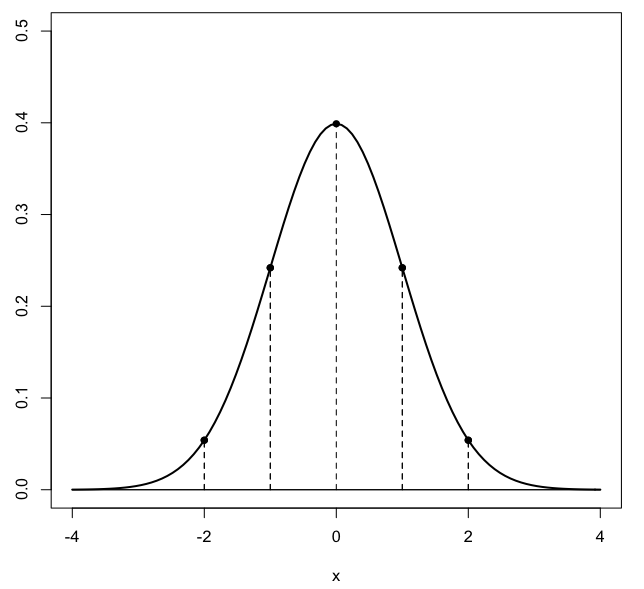
\includegraphics [scale=0.4] {gauss3.png} \end{center}
\begin{document}
\maketitle
\Large

\textbf{RULE III}  If $A(z)$ and $B(z)$ are analytic in a neighborhood of $z_0$, $A(z_0) \ne 0$, and $B(z)$ has a zero at $z_0$ of order 1, then
\[ f(z) = \frac{A(z)}{B(z)} \]
has a pole of first order at $z_0$ and
\[ \text{Res } [f(z),z_0] = \frac{A(z_0)}{B'(z_0)} \]
\subsection*{example}
\[ f(z) = \frac{1}{z^2 + 1} = \frac{1}{(z - i)(z + i)} \]
\[ B = z^2 + 1, \ \ \ B' = 2z \]
\[ \text{Res } [f(z),z=i] = \frac{1}{2i} \]
\[ \text{Res } [f(z),z=-i] = -\frac{1}{2i} \]

\subsection*{example}
\[ f(z) = \frac{z e^z}{z^2 - 1} \]
Both top and bottom are analytic.  The poles of $B(z)$ are at $\pm \ 1$.  $A(z) \ne 0$ at those points.  We have 
\[ \frac{A(z)}{B'(z)} = \frac{z e^z}{2z} \]
\[ \frac{z e^z}{2z} \ \bigg |_{z=1} = \frac{e}{2} \]
\[ \frac{z e^z}{2z} \ \bigg |_{z=-1} = e^{-1} \]

\textbf{RULE IV}  If $A(z)$ and $B(z)$ are analytic in a neighborhood of $z_0$, $A(z_0) \ne 0$, and $B(z)$ has a zero at $z_0$ of order 2, then
\[ \text{Res } [f(z),z_0] = \frac{6A' B'' - 2AB'''}{3B''^2} \]

\subsection*{example}
\[ f(z) = \frac{e^z}{z(z-1)^2} \]
\[ B = z(z^2 - 2z + 1) = z^3 - 2z^2 + z \]
\[ B' = 3z^2 - 4z + 1 \]
\[ B'' = 6z - 4 \]
\[ B''' = 6 \]
So
\[ \frac{6A' B'' - 2AB'''}{3B''^2} = \frac{6(e^z)(6z-4) - 2e^z(6)}{3(6z-4)^2} \ \]
Evaluate at $z=1$:
\[ \frac{6e(2) - 2e(6)}{12} = 0 \]
So only the pole at $z=0$ contributes.


\end{document}  
